% Options for packages loaded elsewhere
\PassOptionsToPackage{unicode}{hyperref}
\PassOptionsToPackage{hyphens}{url}
\PassOptionsToPackage{dvipsnames,svgnames,x11names}{xcolor}
%
\documentclass[
  11pt,
  letterpaper,
]{article}
\usepackage{amsmath,amssymb}
\usepackage{iftex}
\ifPDFTeX
  \usepackage[T1]{fontenc}
  \usepackage[utf8]{inputenc}
  \usepackage{textcomp} % provide euro and other symbols
\else % if luatex or xetex
  \usepackage{unicode-math} % this also loads fontspec
  \defaultfontfeatures{Scale=MatchLowercase}
  \defaultfontfeatures[\rmfamily]{Ligatures=TeX,Scale=1}
\fi
\usepackage{lmodern}
\ifPDFTeX\else
  % xetex/luatex font selection
\fi
% Use upquote if available, for straight quotes in verbatim environments
\IfFileExists{upquote.sty}{\usepackage{upquote}}{}
\IfFileExists{microtype.sty}{% use microtype if available
  \usepackage[]{microtype}
  \UseMicrotypeSet[protrusion]{basicmath} % disable protrusion for tt fonts
}{}
\makeatletter
\@ifundefined{KOMAClassName}{% if non-KOMA class
  \IfFileExists{parskip.sty}{%
    \usepackage{parskip}
  }{% else
    \setlength{\parindent}{0pt}
    \setlength{\parskip}{6pt plus 2pt minus 1pt}}
}{% if KOMA class
  \KOMAoptions{parskip=half}}
\makeatother
\usepackage{xcolor}
\usepackage[margin=1in]{geometry}
\usepackage{longtable,booktabs,array}
\usepackage{calc} % for calculating minipage widths
% Correct order of tables after \paragraph or \subparagraph
\usepackage{etoolbox}
\makeatletter
\patchcmd\longtable{\par}{\if@noskipsec\mbox{}\fi\par}{}{}
\makeatother
% Allow footnotes in longtable head/foot
\IfFileExists{footnotehyper.sty}{\usepackage{footnotehyper}}{\usepackage{footnote}}
\makesavenoteenv{longtable}
\usepackage{graphicx}
\makeatletter
\def\maxwidth{\ifdim\Gin@nat@width>\linewidth\linewidth\else\Gin@nat@width\fi}
\def\maxheight{\ifdim\Gin@nat@height>\textheight\textheight\else\Gin@nat@height\fi}
\makeatother
% Scale images if necessary, so that they will not overflow the page
% margins by default, and it is still possible to overwrite the defaults
% using explicit options in \includegraphics[width, height, ...]{}
\setkeys{Gin}{width=\maxwidth,height=\maxheight,keepaspectratio}
% Set default figure placement to htbp
\makeatletter
\def\fps@figure{htbp}
\makeatother
\setlength{\emergencystretch}{3em} % prevent overfull lines
\providecommand{\tightlist}{%
  \setlength{\itemsep}{0pt}\setlength{\parskip}{0pt}}
\setcounter{secnumdepth}{-\maxdimen} % remove section numbering
% definitions for citeproc citations
\NewDocumentCommand\citeproctext{}{}
\NewDocumentCommand\citeproc{mm}{%
  \begingroup\def\citeproctext{#2}\cite{#1}\endgroup}
\makeatletter
 % allow citations to break across lines
 \let\@cite@ofmt\@firstofone
 % avoid brackets around text for \cite:
 \def\@biblabel#1{}
 \def\@cite#1#2{{#1\if@tempswa , #2\fi}}
\makeatother
\newlength{\cslhangindent}
\setlength{\cslhangindent}{1.5em}
\newlength{\csllabelwidth}
\setlength{\csllabelwidth}{3em}
\newenvironment{CSLReferences}[2] % #1 hanging-indent, #2 entry-spacing
 {\begin{list}{}{%
  \setlength{\itemindent}{0pt}
  \setlength{\leftmargin}{0pt}
  \setlength{\parsep}{0pt}
  % turn on hanging indent if param 1 is 1
  \ifodd #1
   \setlength{\leftmargin}{\cslhangindent}
   \setlength{\itemindent}{-1\cslhangindent}
  \fi
  % set entry spacing
  \setlength{\itemsep}{#2\baselineskip}}}
 {\end{list}}
\usepackage{calc}
\newcommand{\CSLBlock}[1]{\hfill\break\parbox[t]{\linewidth}{\strut\ignorespaces#1\strut}}
\newcommand{\CSLLeftMargin}[1]{\parbox[t]{\csllabelwidth}{\strut#1\strut}}
\newcommand{\CSLRightInline}[1]{\parbox[t]{\linewidth - \csllabelwidth}{\strut#1\strut}}
\newcommand{\CSLIndent}[1]{\hspace{\cslhangindent}#1}
\ifLuaTeX
  \usepackage{selnolig}  % disable illegal ligatures
\fi
\usepackage{bookmark}
\IfFileExists{xurl.sty}{\usepackage{xurl}}{} % add URL line breaks if available
\urlstyle{same}
\hypersetup{
  pdftitle={A National Roadmap for Quantum Technologies: Strategic Infrastructure, Sovereign Capability, and Research Priorities for 2025-2035},
  pdfauthor={Edgar Valdés, Hadox Research Labs},
  colorlinks=true,
  linkcolor={blue},
  filecolor={blue},
  citecolor={blue},
  urlcolor={blue},
  pdfcreator={LaTeX via pandoc}}

\title{A National Roadmap for Quantum Technologies: Strategic
Infrastructure, Sovereign Capability, and Research Priorities for
2025-2035\thanks{Prepared for the Quantum Technologies track of the
twenty-third edition of the Global Information Technology Management
Association Annual Conference, Monterrey, Mexico, May 6-8, 2026, for
which Edgar Antonio Valdés Porras serves as Track Chair. The author
gratefully acknowledges Rogelio Marín and the Centro de Investigación en
Matemáticas, A.C. for intellectual support and institutional context.
All interpretations and remaining errors are the author's
responsibility.}}
\author{Edgar Valdés, Hadox Research Labs}
\date{April 2026}

\begin{document}
\maketitle

\section{Abstract}\label{abstract}

Quantum technologies have become a strategic domain of national
innovation policy because they affect computation, measurement,
cybersecurity, communications, defence, materials science, and
scientific instrumentation. A national roadmap for the 2025-2035 horizon
is developed from enterprise-adoption research, national innovation
systems theory, OECD policy data, NIST/NSA/CISA cybersecurity guidance,
OECD-EPO patent mapping, OpenAlex bibliometrics, and high-performance
computing (HPC) integration studies. The evidence indicates that
national quantum readiness is constrained not only by hardware maturity
but also by institutional capacity, technical workforce formation,
validated use cases, public procurement discipline, cryptographic
migration, HPC-QC workflow capability, and standards participation. The
proposed roadmap distinguishes near-term adoption imperatives,
especially post-quantum cryptography and quantum sensing pilots, from
medium-term testbed and supply-chain development and long-term frontier
research in logical qubits, quantum repeaters, metrology,
device-independent security, and foundations. National quantum
strategies are more coherently evaluated through the accumulation of
absorptive capacity than through symbolic hardware acquisition: the
ability to understand, test, procure, secure, regulate, and eventually
produce quantum technologies.

\textbf{Keywords:} national quantum strategy, quantum technologies,
post-quantum cryptography, quantum sensing, quantum computing,
high-performance computing, HPC-QC integration, innovation policy,
public procurement, strategic infrastructure

\section{1. Introduction}\label{introduction}

Quantum technologies now occupy a position similar to earlier strategic
technologies such as semiconductors, aerospace, telecommunications, and
artificial intelligence. They are not only scientific instruments or
commercial products; they are enabling systems that may reshape
security, measurement, computation, and industrial research. For that
reason, the design of national quantum strategy cannot be reduced to
research funding or startup promotion. It requires an integrated view of
scientific capacity, industrialization, cybersecurity, standards,
procurement, workforce, and international positioning.

The roadmap addresses the 2025-2035 horizon. The analysis is motivated
by a central policy problem: the countries most likely to benefit from
quantum technologies will not necessarily be those that announce the
largest hardware ambitions, but those that build absorptive capacity
before markets mature. Absorptive capacity refers here to the
institutional ability to evaluate quantum claims, identify use cases,
train personnel, migrate cryptographic systems, deploy early sensing
applications, participate in supply chains, and maintain frontier
research links.

Four research questions structure the analysis. First, what does the
current evidence reveal about quantum readiness at the organizational
and national levels? Second, which quantum domains are most appropriate
for near-term, medium-term, and long-term policy intervention? Third,
what institutional architecture can support a national quantum
transition without overcommitting to immature hardware pathways? Fourth,
how should high-performance computing systems mediate early quantum
computing adoption?

\section{2. Evidence Base and Method}\label{evidence-base-and-method}

The study uses a research synthesis design. Its theoretical frame draws
on absorptive capacity, national innovation systems, innovation
diffusion, and mission-oriented policy (\citeproc{ref-cohen1990}{Cohen
and Levinthal 1990}; \citeproc{ref-lundvall1992}{Lundvall 1992};
\citeproc{ref-nelson1993}{Nelson 1993}; \citeproc{ref-rogers2003}{Rogers
2003}; \citeproc{ref-mazzucato2018}{Mazzucato 2018}). This frame treats
quantum readiness as an institutional capability rather than as a linear
consequence of scientific progress. The synthesis also treats quantum
computing as part of an HPC-QC continuum rather than as an isolated
successor to classical supercomputing. The adoption layer is anchored in
Kwon et al. (\citeproc{ref-kwon2026}{2026}), which analyzes enterprise
intention to adopt quantum computing through expert interviews and a
survey of 250 IT decision-makers. The policy layer relies on OECD
reports on national quantum strategies and business readiness. OECD
reports approximately USD 55.7 billion in announced public quantum
commitments worldwide since 2013 and USD 11.235 billion PPP in 12,209
quantum-related R\&D awards between 2015 and 2023 across 19 OECD members
and EU-EC programmes (\citeproc{ref-oecd2025a}{OECD 2025a},
\citeproc{ref-oecd2026}{2026}). The security layer uses NIST, NSA, and
CISA guidance, especially the 2024 NIST post-quantum cryptography
standards and critical-infrastructure migration guidance
(\citeproc{ref-cisaNistNsa2022}{CISA, NIST, and NSA 2022};
\citeproc{ref-nist2024}{NIST 2024}; \citeproc{ref-nsa2024}{NSA 2024}).

OpenAlex bibliometric data serve as a proxy for scientific absorptive
capacity.\footnote{Adoption proxies are used because comprehensive
  public data on direct quantum deployment remain unavailable. Funding,
  publications, patents, readiness surveys, and standards activity
  measure different dimensions of capability and should not be
  interpreted as interchangeable indicators.} The query for the concept
``Quantum technology'' from 2015 to 2025 returns 15,279 works in the
extracted concept set. The leading country affiliations in the extract
are the United States, China, Germany, the United Kingdom, and France.
Bibliometric data are not treated as direct adoption metrics; they
approximate the distribution of research capacity that can support
future adoption.

\begin{figure}
\centering
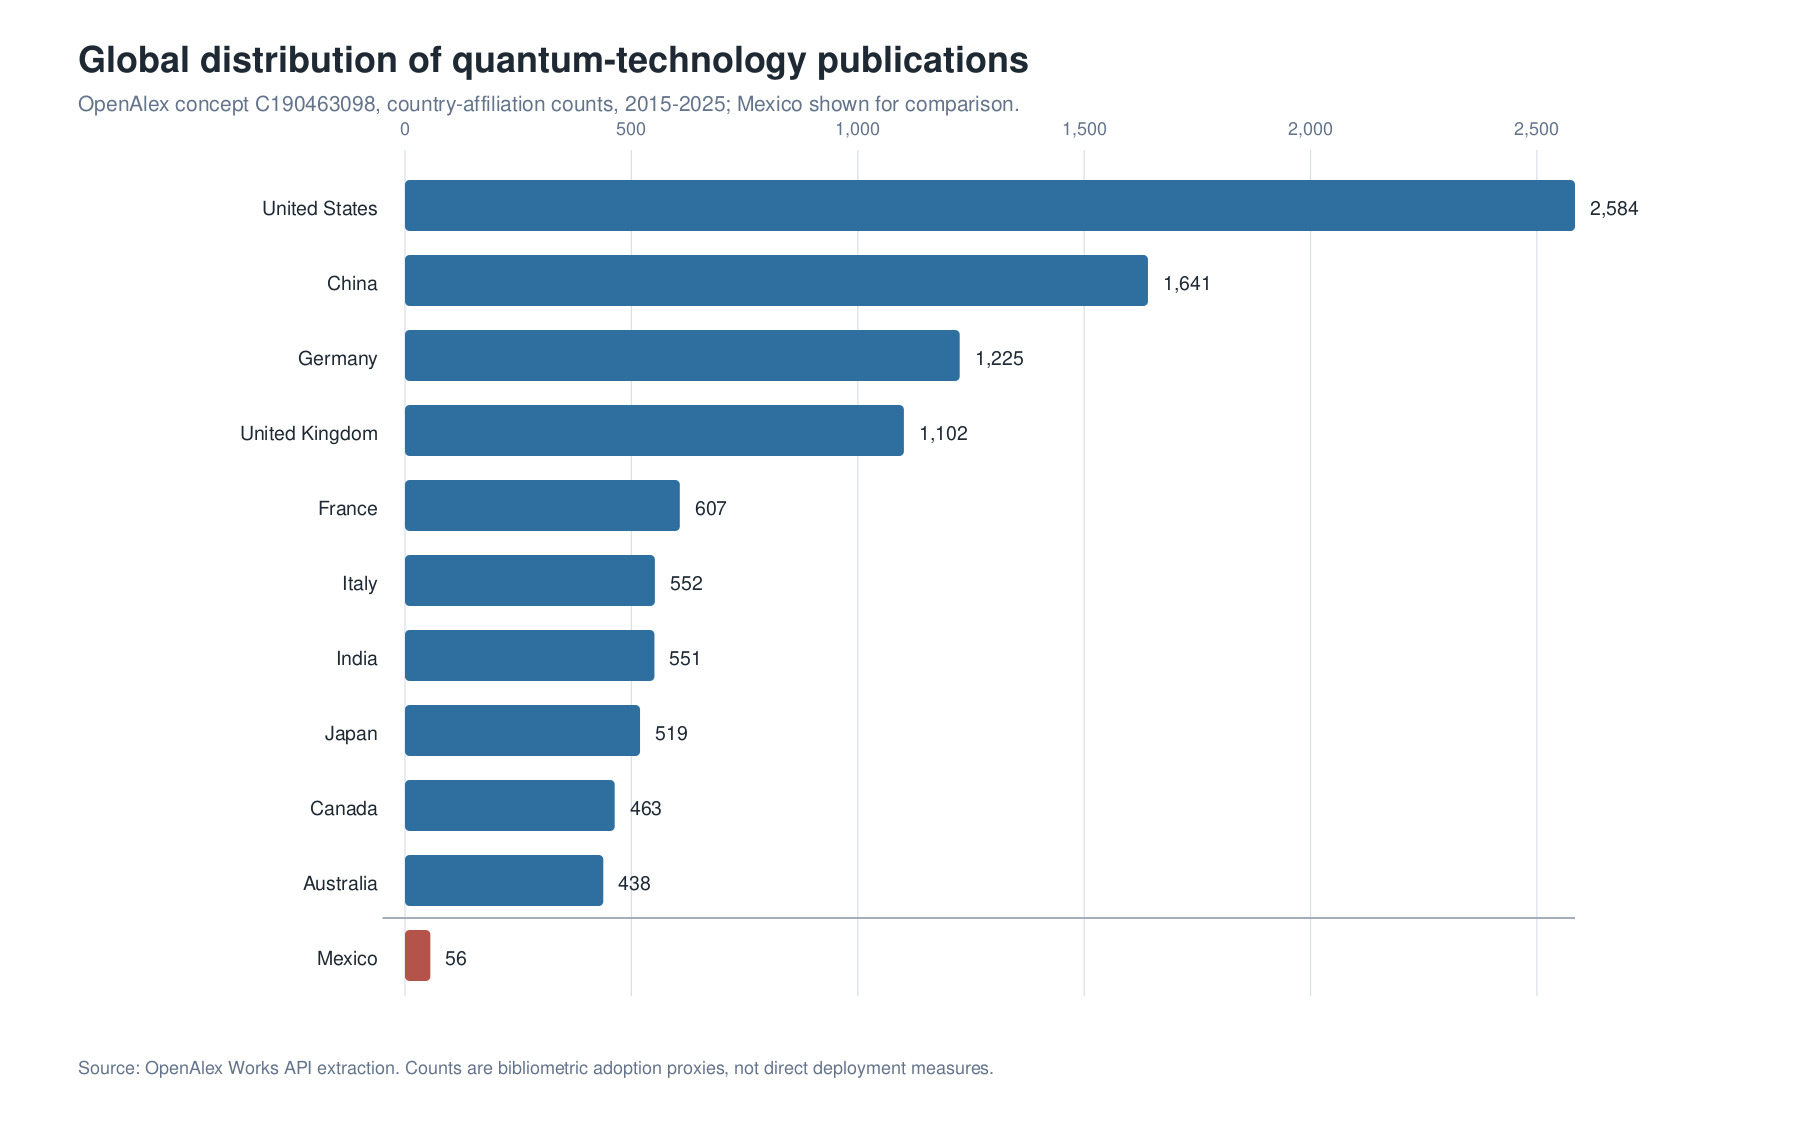
\includegraphics[width=0.95\textwidth,height=\textheight]{figures/fig1_global_country_distribution.png}
\caption{Global distribution of quantum-technology publication capacity.
OpenAlex country-affiliation counts for the concept ``Quantum
technology'' show a concentrated geography led by the United States,
China, Germany, the United Kingdom, and France, with Mexico included as
a comparison case. Counts are interpreted as scientific
absorptive-capacity proxies rather than direct deployment indicators.}
\end{figure}

\section{3. Results: The Structure of the Readiness
Gap}\label{results-the-structure-of-the-readiness-gap}

The international evidence shows a consistent disjunction between
expected quantum impact and institutional preparation. Kwon et al.
(\citeproc{ref-kwon2026}{2026}) find that adoption intention increases
with perceived quantum advantage, belief in quantum superiority, budget
continuity, regulatory support, and co-creation capacity, while
resistance and financial risk reduce adoption intent. OECD readiness
data show a similar pattern across sectors: executives expect quantum
technologies to matter, but many organizations lack readiness plans,
dedicated budgets, and validated use cases.

\begin{longtable}[]{@{}
  >{\raggedright\arraybackslash}p{(\columnwidth - 4\tabcolsep) * \real{0.3333}}
  >{\raggedright\arraybackslash}p{(\columnwidth - 4\tabcolsep) * \real{0.3333}}
  >{\raggedright\arraybackslash}p{(\columnwidth - 4\tabcolsep) * \real{0.3333}}@{}}
\toprule\noalign{}
\begin{minipage}[b]{\linewidth}\raggedright
Evidence source
\end{minipage} & \begin{minipage}[b]{\linewidth}\raggedright
Quantitative evidence
\end{minipage} & \begin{minipage}[b]{\linewidth}\raggedright
Interpretation
\end{minipage} \\
\midrule\noalign{}
\endhead
\bottomrule\noalign{}
\endlastfoot
Kwon et al. (\citeproc{ref-kwon2026}{2026}) & 250 IT decision-makers and
11 expert interviews & Adoption depends on perceived advantage, budget
continuity, regulatory support, and co-creation \\
OECD national strategies & USD 55.7 billion in announced public
commitments since 2013 & Quantum technologies have become a state-level
strategic competition \\
OECD Fundstat & USD 11.235 billion PPP in 12,209 R\&D awards, 2015-2023
& Public research investment is increasingly coordinated \\
OECD readiness surveys & High expected disruption but limited strategic
planning and budgets & Awareness does not automatically produce
readiness \\
OECD-EPO mapping & 31,700 mapped quantum patent families, 2005-2024 &
Technological invention is measurable and geographically concentrated \\
OpenAlex & 15,279 quantum-technology works, 2015-2025 query & Scientific
absorptive capacity is unevenly distributed \\
NIST PQC standards & ML-KEM, ML-DSA, and SLH-DSA finalized in 2024 & PQC
migration is already an implementation agenda \\
\end{longtable}

The readiness gap has three dimensions. The first is organizational:
firms and agencies lack internal quantum literacy, budgets, and use-case
development processes. The second is infrastructural: testbeds,
standards laboratories, cryptographic inventories, and procurement rules
are underdeveloped. The third is strategic: countries face choices about
which capabilities to build domestically, which to access through
alliances or cloud platforms, and which to monitor as frontier science.

\begin{figure}
\centering
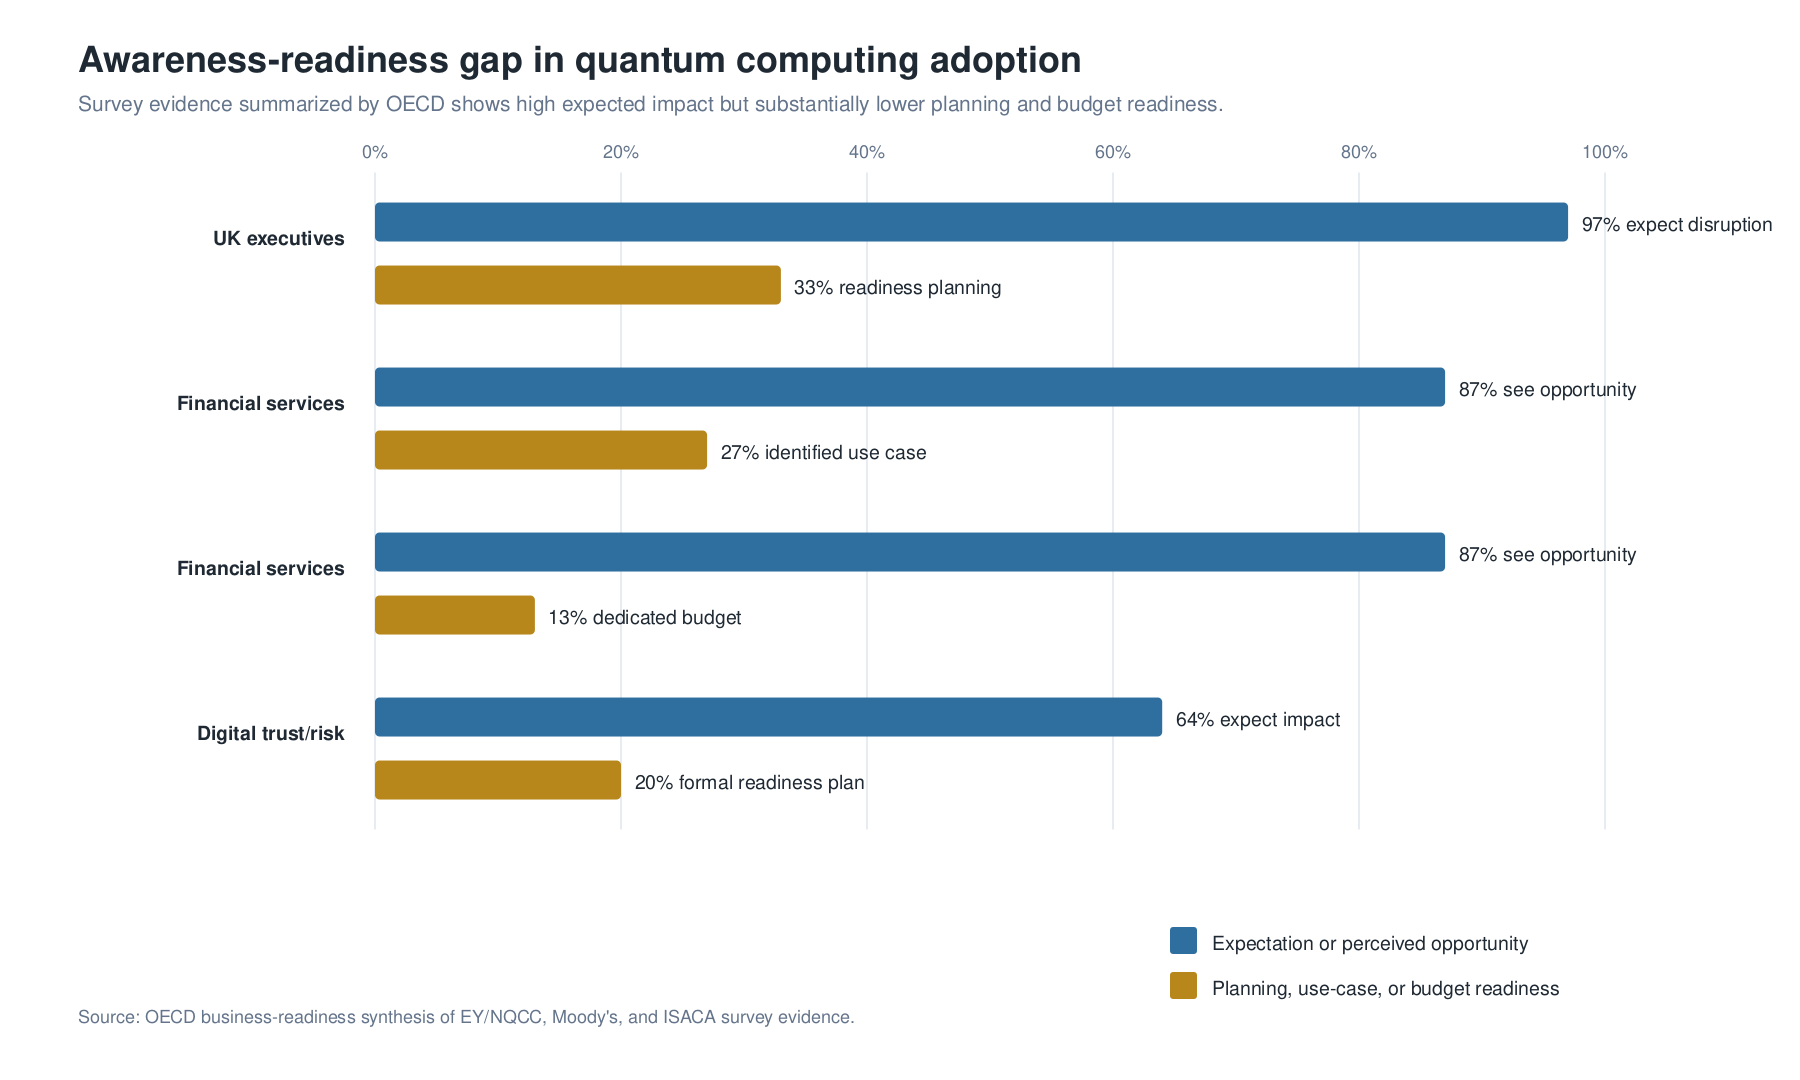
\includegraphics[width=0.95\textwidth,height=\textheight]{figures/fig3_readiness_gap.png}
\caption{Awareness-readiness gap in quantum computing adoption. Survey
evidence summarized by OECD indicates that high expected impact coexists
with substantially lower levels of planning, use-case definition, and
dedicated budget formation.}
\end{figure}

\section{4. A National Capability
Model}\label{a-national-capability-model}

The evidence supports a five-pillar capability model.

\textbf{Scientific frontier.} National strategy requires sustained
research in quantum information science, materials, photonics,
metrology, algorithms, error correction, and foundations. This pillar
creates long-term autonomy and supports participation in international
research networks.

\textbf{Industrialization.} Industrial policy depends on realistic
positions in the quantum value chain: quantum software, control systems,
sensing integration, photonics, component testing, calibration,
cryogenic services, cybersecurity, and metrology.

\textbf{Security and sovereignty.} The immediate policy priority is
post-quantum cryptography migration. Quantum key distribution may be
appropriate for selected high-value links, but it is evaluated here as
specialized infrastructure rather than as a general substitute for PQC.

\textbf{Workforce.} The workforce problem extends beyond PhD-level
physics. It includes technicians, engineers, cybersecurity
professionals, procurement officers, and executives capable of
operating, evaluating, and governing quantum systems
(\citeproc{ref-kaur2022}{Kaur and Venegas-Gomez 2022}).

\textbf{Governance and standards.} Standards, benchmarks, and public
procurement rules are necessary to prevent quantum washing and to align
public expenditure with measurable technological performance.

\begin{figure}
\centering
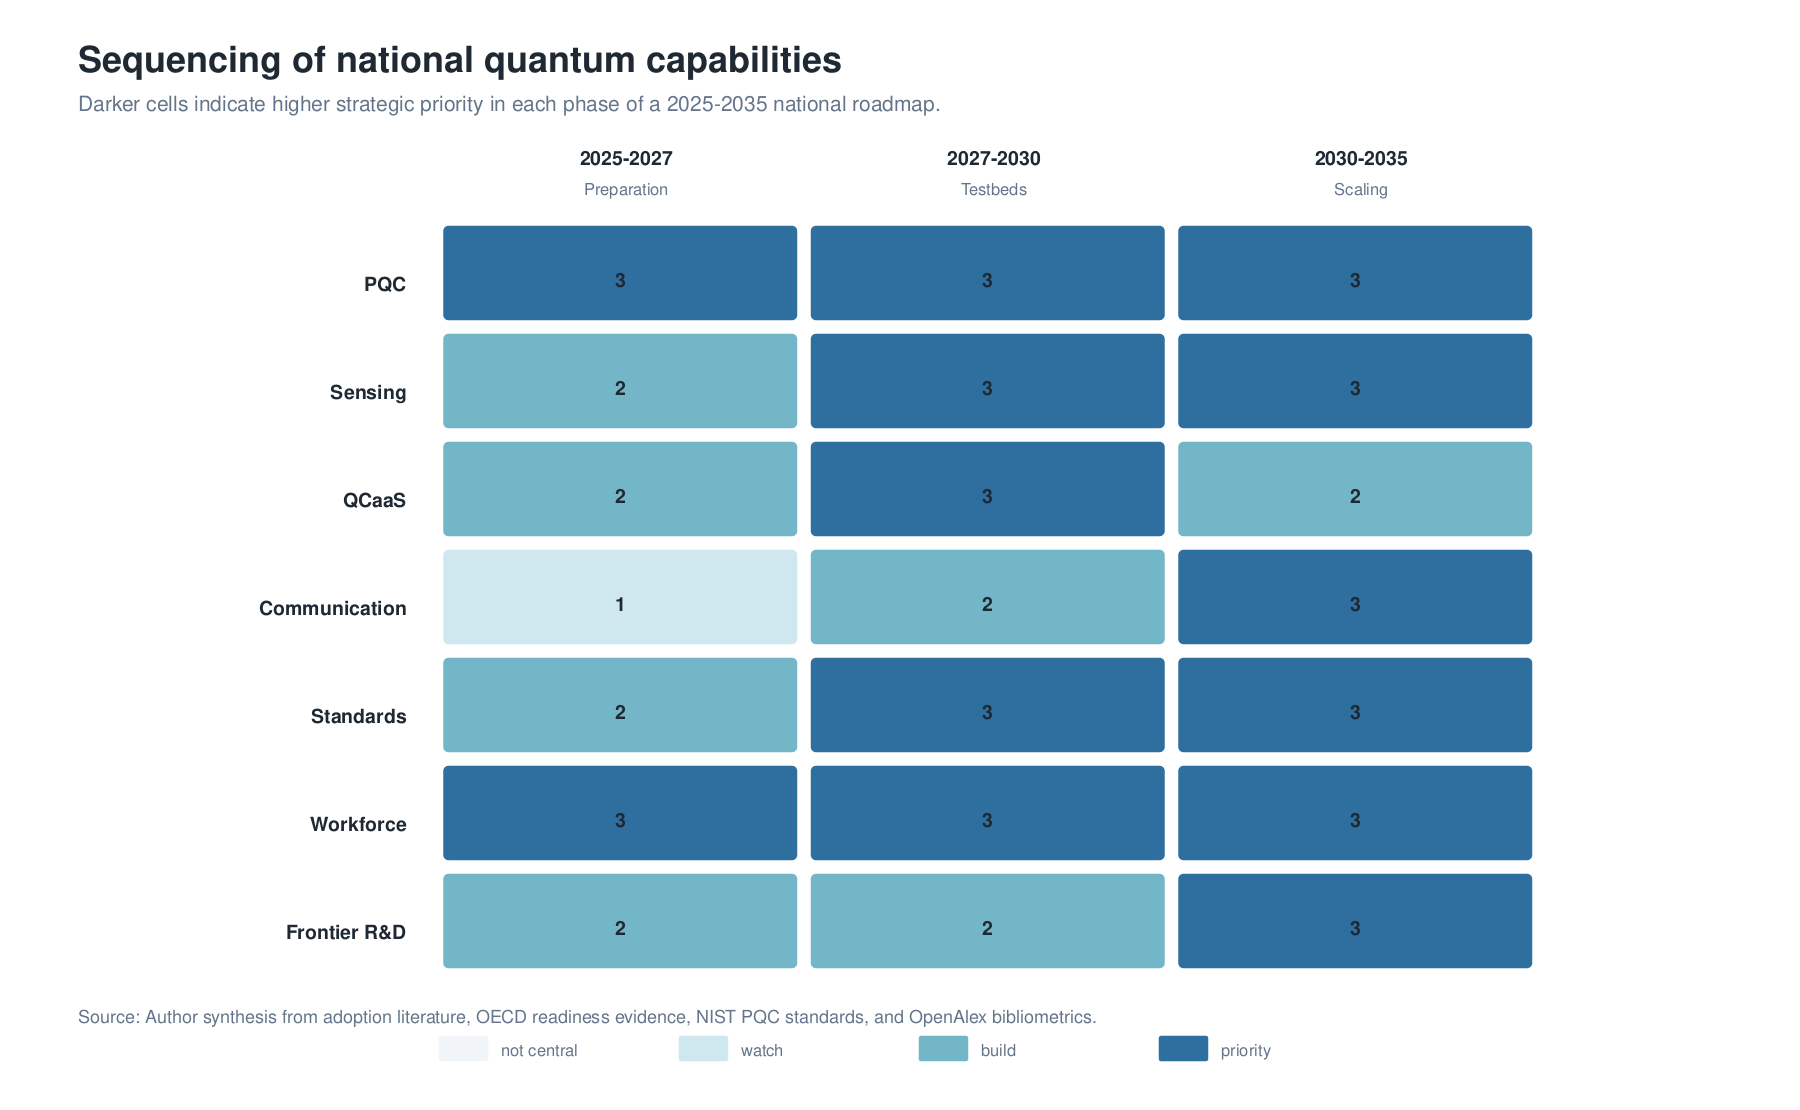
\includegraphics[width=0.95\textwidth,height=\textheight]{figures/fig4_capability_heatmap.png}
\caption{Sequencing of national quantum capabilities. The heatmap scores
strategic priority across three roadmap phases, emphasizing that PQC,
workforce, standards, sensing, QCaaS, communication, and frontier R\&D
mature on different policy timelines.}
\end{figure}

\section{5. Roadmap 2025-2035}\label{roadmap-2025-2035}

The roadmap is organized as a sequence of national capabilities rather
than a linear prediction of hardware breakthroughs.

\begin{longtable}[]{@{}
  >{\raggedright\arraybackslash}p{(\columnwidth - 6\tabcolsep) * \real{0.2500}}
  >{\raggedright\arraybackslash}p{(\columnwidth - 6\tabcolsep) * \real{0.2500}}
  >{\raggedright\arraybackslash}p{(\columnwidth - 6\tabcolsep) * \real{0.2500}}
  >{\raggedright\arraybackslash}p{(\columnwidth - 6\tabcolsep) * \real{0.2500}}@{}}
\toprule\noalign{}
\begin{minipage}[b]{\linewidth}\raggedright
Period
\end{minipage} & \begin{minipage}[b]{\linewidth}\raggedright
Strategic emphasis
\end{minipage} & \begin{minipage}[b]{\linewidth}\raggedright
Institutional actions
\end{minipage} & \begin{minipage}[b]{\linewidth}\raggedright
Expected capability
\end{minipage} \\
\midrule\noalign{}
\endhead
\bottomrule\noalign{}
\endlastfoot
2025-2027 & Preparation and security & Cryptographic inventories, PQC
pilots, quantum readiness office, QCaaS and HPC-QC access, workforce
curricula, sensing feasibility studies & Baseline institutional
awareness and early security migration \\
2027-2030 & Testbeds and early deployment & Sensing pilots, standards
laboratory, procurement protocols, QKD pilots where justified, supplier
mapping, applied research consortia, HPC-QC workflow pilots &
Operational learning and validated early applications \\
2030-2035 & Selective scaling and frontier integration & Logical-qubit
readiness, quantum network experiments, advanced metrology, supply-chain
specialization, frontier research centres, HPC-QC scaling & Domestic
absorptive capacity connected to global frontier \\
\end{longtable}

The sequence reflects the maturity differences among quantum domains.
PQC and sensing can be pursued before fault-tolerant quantum computing.
QCaaS can support learning before domestic hardware exists. Quantum
communication testbeds can be developed before national-scale networks.
Frontier research can proceed in parallel as a long-term option
generator.

\begin{figure}
\centering
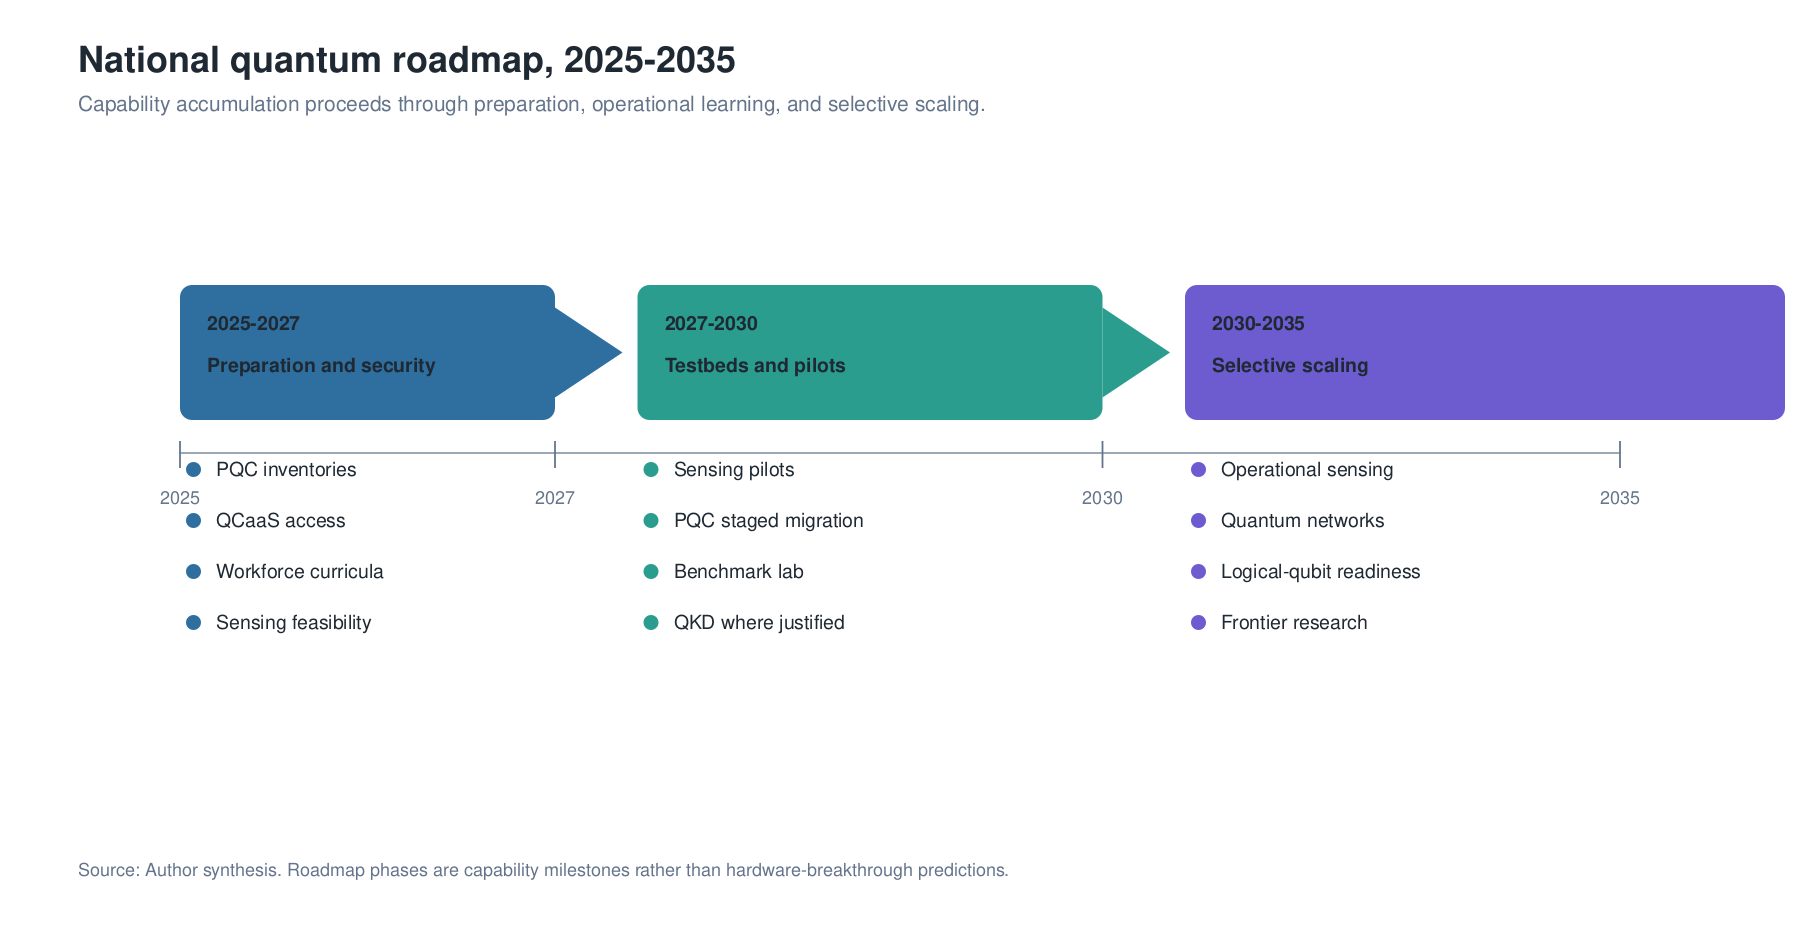
\includegraphics[width=0.95\textwidth,height=\textheight]{figures/fig5_roadmap_timeline.png}
\caption{Roadmap for national quantum capability formation, 2025-2035.
The sequence is organized around institutional readiness, operational
learning, and selective scaling rather than prediction of a single
hardware breakthrough.}
\end{figure}

\section{6. Institutional
Architecture}\label{institutional-architecture}

The roadmap requires institutional coordination. A National Quantum
Office coordinates policy, funding, international partnerships, and
performance monitoring. A Post-Quantum Cryptography Task Force manages
cryptographic inventories, prioritization, and migration schedules. A
National Quantum Testbed Network connects universities, agencies, firms,
and infrastructure operators. A Quantum Standards and Benchmarking
Laboratory evaluates claims, interoperability, security, and procurement
metrics. A Quantum Workforce Council aligns educational programmes with
expected demand. A Frontier Quantum Research Fund supports high-risk
work in error correction, metrology, repeaters, foundations, and
measurement science.

The purpose of this architecture is not bureaucratic expansion. It is
coordination under uncertainty. Quantum technologies are difficult to
evaluate because performance claims are highly technical, market
forecasts are volatile, and hardware trajectories remain contested.
Public institutions therefore need evaluation capacity before
procurement scales.

\section{7. Strategic Domains}\label{strategic-domains}

Post-quantum cryptography is the first national adoption domain because
it addresses long-lived security risk and is already supported by
standards. The transition requires asset inventories, crypto-agility,
staged migration, vendor coordination, and critical-infrastructure
governance.

Quantum sensing is the strongest near-term public-value domain. Sensing
applications can target geodesy, infrastructure monitoring, underground
water, navigation, health, mining, energy systems, and environmental
risk. These pilots can generate measurable value and build engineering
capacity.

Quantum computing initially functions as a learning and benchmarking
domain. QCaaS access allows universities, agencies, and firms to test
algorithms without owning immature hardware. The relevant output is not
immediate advantage but organizational competence.

High-performance computing is the transition layer for quantum
computing. In this model, quantum processing units operate as potential
accelerators embedded in HPC workflows, while classical systems handle
data preparation, scheduling, error mitigation, verification, and
post-processing (\citeproc{ref-cranganore2024}{Cranganore et al. 2024};
\citeproc{ref-beck2024}{Beck et al. 2024}; \citeproc{ref-liu2024}{Liu et
al. 2024}). HPC centers therefore become early quantum adoption
institutions even before domestic quantum hardware exists. Their role is
to connect quantum software experiments to scientific codes, data
infrastructure, reproducible workflows, and classical baselines.

Quantum communication is best developed through targeted testbeds.
Repeater technologies, memories, entanglement distribution, and
device-independent security are important frontier areas, while wide
deployment depends on operational evidence and cost-benefit analysis.

\section{8. Discussion}\label{discussion}

The roadmap implies that national quantum strategy is more coherently
evaluated by capability accumulation than by headline hardware
acquisition. This distinction is important because premature hardware
procurement can create dependency, while readiness programmes create
optionality. Countries that develop cryptographic migration capacity,
sensing testbeds, HPC-QC workflow capacity, workforce pathways, and
standards laboratories will be better positioned to adopt quantum
technologies regardless of which hardware modality prevails.

The roadmap also rejects a false choice between near-term applications
and foundational science. Near-term applications generate institutional
learning and public value. Frontier research generates long-term
scientific autonomy, instrumentation, and human capital. A robust
strategy requires both layers.

\section{9. Acknowledgments}\label{acknowledgments}

This manuscript was prepared for the Quantum Technologies track of the
twenty-third edition of the Global Information Technology Management
Association Annual Conference, Monterrey, Mexico, May 6-8, 2026. The
author acknowledges his role as Track Chair for Quantum Technologies and
gratefully acknowledges Rogelio Marín and the Centro de Investigación en
Matemáticas, A.C. for intellectual support and institutional context.
All interpretations and remaining errors are the author's
responsibility.

\section{10. Data Availability}\label{data-availability}

The quantitative evidence underlying this roadmap is drawn from OECD
public reports, NIST/NSA/CISA guidance, OECD-EPO patent mapping, and
OpenAlex bibliometric queries. Processed OpenAlex CSV extracts used for
country and year counts are deposited in the companion research
repository.

\section{11. Code Availability}\label{code-availability}

The companion research repository contains the source manuscript,
processed data, BibTeX bibliography, figure-generation code, and
reproducible build script used to generate the manuscript outputs. The
repository is intended to support inspection of the OpenAlex extracts,
regeneration of figures, and reconstruction of the PDF, TeX, and DOCX
versions from the manuscript sources.

\section{12. Limitations}\label{limitations}

The analysis relies on adoption proxies rather than direct deployment
data. Funding, publications, patents, standards, and readiness surveys
measure different dimensions of quantum capacity and are not
interchangeable. A future empirical extension would require national
surveys of firms, agencies, and infrastructure operators.

\section{13. Competing Interests}\label{competing-interests}

The author declares no competing interests.

\section{References}\label{references}

\phantomsection\label{refs}
\begin{CSLReferences}{1}{0}
\bibitem[\citeproctext]{ref-beck2024}
Beck, Thomas, Alessandro Baroni, Ryan Bennink, Gilles Buchs, Eduardo
Antonio Coello Perez, Markus Eisenbach, Rafael Ferreira da Silva, et al.
2024. {``Integrating Quantum Computing Resources into Scientific HPC
Ecosystems.''} \emph{Future Generation Computer Systems}.
\url{https://doi.org/10.1016/j.future.2024.06.058}.

\bibitem[\citeproctext]{ref-bova2020}
Bova, Francesco, Avi Goldfarb, and Roger G. Melko. 2020. {``The Emerging
Commercial Landscape of Quantum Computing.''} \emph{Nature Reviews
Physics} 2: 596--98. \url{https://doi.org/10.1038/s42254-020-00247-5}.

\bibitem[\citeproctext]{ref-cisaNistNsa2022}
CISA, NIST, and NSA. 2022. {``Preparing Critical Infrastructure for
Post-Quantum Cryptography.''}
\url{https://www.cisa.gov/sites/default/files/2022-09/cisa_insight_post_quantum_cryptography_508.pdf}.

\bibitem[\citeproctext]{ref-cohen1990}
Cohen, Wesley M., and Daniel A. Levinthal. 1990. {``Absorptive Capacity:
A New Perspective on Learning and Innovation.''} \emph{Administrative
Science Quarterly} 35 (1): 128--52.
\url{https://doi.org/10.2307/2393553}.

\bibitem[\citeproctext]{ref-cranganore2024}
Cranganore, Sandeep Suresh, Vincenzo De Maio, Ivona Brandic, and Ewa
Deelman. 2024. {``Paving the Way to Hybrid Quantum-Classical Scientific
Workflows.''} \emph{Future Generation Computer Systems} 158: 346--66.
\url{https://doi.org/10.1016/j.future.2024.04.030}.

\bibitem[\citeproctext]{ref-kaur2022}
Kaur, Maninder, and Alberto Venegas-Gomez. 2022. {``Defining the Quantum
Workforce Landscape: A Review of Global Quantum Education
Initiatives.''} \emph{Optical Engineering} 61 (8): 081806.
\url{https://doi.org/10.1117/1.OE.61.8.081806}.

\bibitem[\citeproctext]{ref-kwon2026}
Kwon, Ohbyung, Seongjun Kwon, Timothy Jung, and Saifeddin Alimamy. 2026.
{``Factors Influencing the Adoption Intent of Quantum Computing in
Enterprises: An Innovation Adoption Process Perspective.''}
\emph{International Journal of Information Management} 86: 102978.
\url{https://doi.org/10.1016/j.ijinfomgt.2025.102978}.

\bibitem[\citeproctext]{ref-liu2024}
Liu, Jie, Huan Ma, Honghui Shang, Zhenyu Li, and Jinlong Yang. 2024.
{``Quantum-Centric High Performance Computing for Quantum Chemistry.''}
\emph{Physical Chemistry Chemical Physics} 26: 15831--43.
\url{https://doi.org/10.1039/D4CP00436A}.

\bibitem[\citeproctext]{ref-lundvall1992}
Lundvall, Bengt-Ake, ed. 1992. \emph{National Systems of Innovation:
Toward a Theory of Innovation and Interactive Learning}. London: Pinter.

\bibitem[\citeproctext]{ref-mazzucato2018}
Mazzucato, Mariana. 2018. {``Mission-Oriented Innovation Policies:
Challenges and Opportunities.''} \emph{Industrial and Corporate Change}
27 (5): 803--15. \url{https://doi.org/10.1093/icc/dty034}.

\bibitem[\citeproctext]{ref-nelson1993}
Nelson, Richard R., ed. 1993. \emph{National Innovation Systems: A
Comparative Analysis}. New York: Oxford University Press.

\bibitem[\citeproctext]{ref-nist2024}
NIST. 2024. {``NIST Releases First 3 Finalized Post-Quantum Encryption
Standards.''}
\url{https://www.nist.gov/news-events/news/2024/08/nist-releases-first-3-finalized-post-quantum-encryption-standards}.

\bibitem[\citeproctext]{ref-nsa2024}
NSA. 2024. {``Post-Quantum Cybersecurity Resources.''}
\url{https://www.nsa.gov/Cybersecurity/Post-Quantum-Cybersecurity-Resources/}.

\bibitem[\citeproctext]{ref-oecd2025a}
OECD. 2025a. {``An Overview of National Strategies and Policies for
Quantum Technologies.''} OECD Digital Economy Papers.
\url{https://www.oecd.org/en/publications/an-overview-of-national-strategies-and-policies-for-quantum-technologies_5e55e7ab-en.html}.

\bibitem[\citeproctext]{ref-oecd2025b}
---------. 2025b. {``Mapping the Global Quantum Ecosystem.''}
\url{https://www.oecd.org/content/dam/oecd/en/publications/reports/2025/12/mapping-the-global-quantum-ecosystem_47891dd2/20251217-0001.pdf}.

\bibitem[\citeproctext]{ref-oecd2026}
---------. 2026. {``Building Business Readiness for Quantum
Computing.''} OECD Digital Economy Papers.
\url{https://www.oecd.org/en/publications/building-business-readiness-for-quantum-computing_ee847e5f-en.html}.

\bibitem[\citeproctext]{ref-openalex2026}
OpenAlex. 2026. {``OpenAlex Works API.''}
\url{https://docs.openalex.org/}.

\bibitem[\citeproctext]{ref-preskill2018}
Preskill, John. 2018. {``Quantum Computing in the NISQ Era and
Beyond.''} \emph{Quantum} 2: 79.
\url{https://doi.org/10.22331/q-2018-08-06-79}.

\bibitem[\citeproctext]{ref-qedc2022}
QED-C. 2022. {``Guide to Building a Quantum Technician Workforce.''}
\url{https://quantumconsortium.org/publication/guide-to-building-a-quantum-technician-workforce-2/}.

\bibitem[\citeproctext]{ref-rogers2003}
Rogers, Everett M. 2003. \emph{Diffusion of Innovations}. 5th ed. New
York: Free Press.

\end{CSLReferences}

\end{document}
